\setlength{\textwidth}{\fullwidth}
\setlength{\evensidemargin}{\oddsidemargin}
\addtolength{\textwidth}{-5truemm}
\addtolength{\oddsidemargin}{5truemm}

%package類
%%%%%%%%%%%%%%%%%%%%
\usepackage[utf8]{inputenc}
\usepackage[T1]{fontenc}
\usepackage[prefernoncjk]{pxcjkcat}
\usepackage[scaled=1.05,helvratio=1.0]{newtxtext}
\usepackage[dvipdfmx]{color}
\usepackage[dvipsnames]{xcolor}
%\usepackage[colorlinks=true,allcolors=blue]{hyperref}
\usepackage[dvipdfmx,hidelinks]{hyperref}
\usepackage{pxjahyper} 
\usepackage{array,amsmath,amssymb,bm,cases} 
\usepackage{graphicx} 
\usepackage{url} 
\usepackage{natbib}
\usepackage{ascmac} 
\usepackage{enumerate}
\usepackage[nottoc,notlot,notlof]{tocbibind}
%\usepackage{mathtools}
\usepackage[nooneline]{subfigure}
\subfiguretopcaptrue 
\usepackage{tcolorbox}

\usepackage{niceframe}

\usepackage{amsthm}
\theoremstyle{definition}
\newtheorem{exmp}{練習問題}[chapter]

\allowdisplaybreaks[4] 

%%%%%%%%%%%%%%%%%%%%
\newcommand{\bs}{\symbol{92}} %backslash
\newcommand{\red}[1]{\textcolor{red}{#1}} %文字色赤
\newcommand{\blue}[1]{\textcolor{blue}{#1}} %文字色青
\newcommand{\green}[1]{\textcolor{green}{#1}} %文字色緑
\newcommand{\rb}[1]{\textcolor{RoyalBlue}{#1}}
\newcommand{\ro}[1]{\textcolor{RedOrange}{#1}}
\newcommand{\ured}[1]{\textcolor{red}{\underline{\textcolor{black}{#1}}}} %下線赤
\newcommand{\ugreen}[1]{\textcolor{green}{\underline{\textcolor{black}{#1}}}} %下線緑
\newcommand{\ublue}[1]{\textcolor{blue}{\underline{\textcolor{black}{#1}}}} %下線青
\newcommand\adndt{Atomic Data and Nuclear Data Tables}
\newcommand\Annual{Annual Review of Nuclear and Particle Science}
\newcommand\aj{The Astronomical Journal}
\newcommand\aap{\rm{A\&A}}
\newcommand\apj{\rm{ApJ}}
\newcommand\apjl{\rm{ApJ, Letter}}
\newcommand\apjs{\rm{ApJ, Supplement}}
\newcommand\araa{\rm{Annual Review of A\& A}}
\newcommand\arxiv{\rm{arXiv e-prints}}
\newcommand\mnras{\rm{MNRAS}}
%\newcommand\Nature{Nature Communications}
\newcommand\Nature{\rm{Nature}}
\newcommand\nat{\rm{Nature}}
\newcommand\nds{Nuclear Data Sheets}
%\newcommand\Science{Science communication}
\newcommand\pasp{PASP}
\newcommand\physrep{Physics Reports}
\newcommand\prl{Physical Review Letters}
\newcommand\rpp{Reports on Progress in Physics}
\newcommand\Science{\rm{Science}}
\newcommand\ssr{Space Science Reviews}
\newcommand\prd{Physical Review D}
\newcommand\pasj{\rm{PASJ}}
\newcommand\sovast{Soviet Astronomy}
\newcommand\aaps{Astronomy and Astrophysics Supplement}
\newcommand\physscr{Physica Scripta}
\newcommand\jqsrt{Journal of Quantitative Spectroscopy \& Radiative Transfer}
%%%%%%%%%%%%%%%%%%%%

\usepackage{listings,jvlisting}
%ここからソースコードの表示に関する設定
\lstset{
  basicstyle={\ttfamily},
  identifierstyle={\small},
  commentstyle={\smallitshape},
  keywordstyle={\small\bfseries},
  ndkeywordstyle={\small},
  stringstyle={\small\ttfamily},
  frame={tb},
  breaklines=true,
  columns=[l]{fullflexible},
  numbers=left,
  xrightmargin=0zw,
  xleftmargin=3zw,
  numberstyle={\scriptsize},
  stepnumber=1,
  numbersep=1zw,
  lineskip=-0.5ex
}
%ここまでソースコードの表示に関する設定


\makeatletter

\newcommand{\subtitle}[1]{\def\@subtitle{#1}}
\renewcommand{\and}{\\}
\renewcommand{\maketitle}{
  \thispagestyle{empty}
  \mbox{}
  \vfill
  \noindent{\Huge\bf \@title}\\
  \rule{\textwidth}{3pt}
  \begin{flushright}
    \vskip -3mm
    \Large{\@subtitle}\\
    \Large{\@date}
  \end{flushright}
  \vfill
  \begin{center}%
  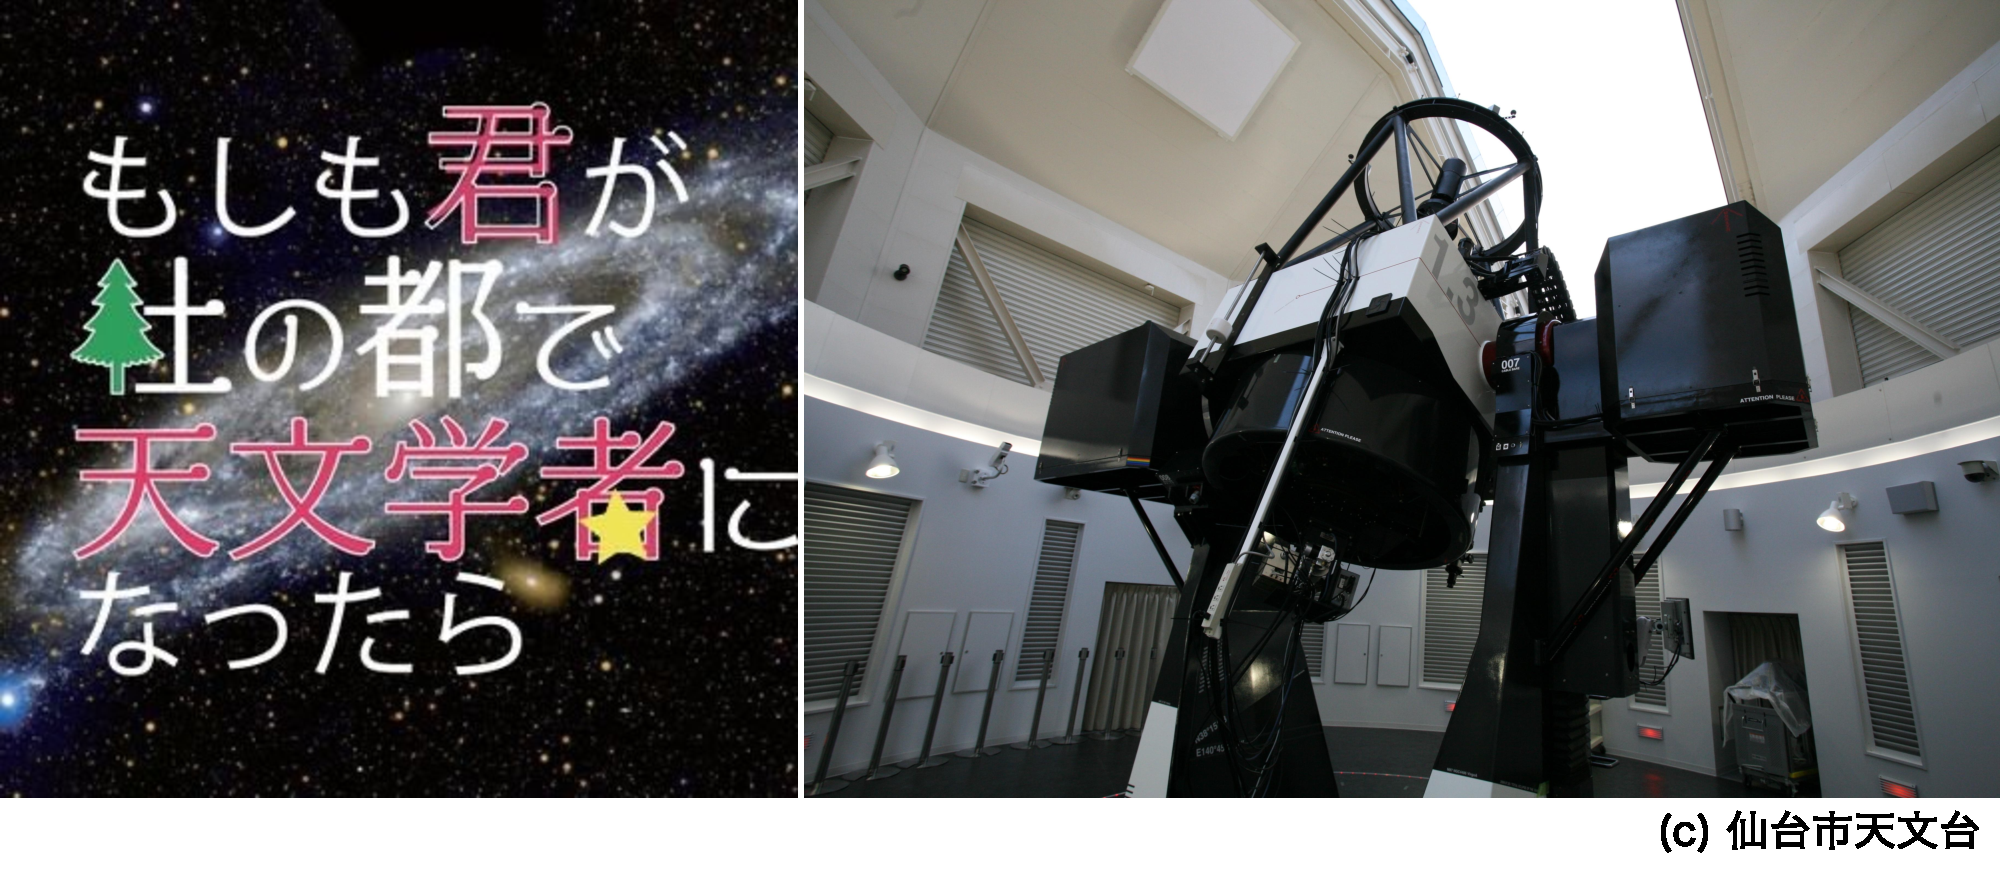
\includegraphics[width=0.98\linewidth]{fig/moshiten.pdf}
  \end{center}%
  \begin{flushleft}
    \bf\LARGE
    \@author
  \end{flushleft}
  \vskip -5mm\rule{\textwidth}{2pt}
  \cleardoublepage
}
\makeatother

\makeatletter
\@addtoreset{equation}{section}
\def\theequation{\thesection.\arabic{equation}}
\makeatother